\documentclass[]{article}
\usepackage[spanish]{babel} 
\usepackage{amsmath} 
\usepackage[colorlinks=true]{hyperref}
\usepackage{enumitem} 
\usepackage{graphicx}   
\usepackage[a4paper,top=3cm,bottom=3cm,left=3cm,right=3cm,marginparwidth=1.75cm]{geometry} 
\usepackage[]{subfigure}
\graphicspath{{./graficos/Lab-Termo/Git/Documentos}} 
\usepackage{float}

%\title{Informe I}
%\author{}
%\date{\today}
%==================================================================================
\begin{document}
\begin{titlepage}
      \begin{center}     
              
            
\includegraphics[width=0.2\textwidth]{graficos/escudo_udec.png}                       %Para poner logo udec   %{nombre carpeta\nombreimagen}
            
            
            
            \vspace{1cm}
            \textsc{{\LARGE Universidad de concepcion}}
            
            \vspace{1cm}
            {\scshape\Large Facultad de ciencias fisícas y matematicas \par}
            \vspace{2cm}
            {\scshape\Huge Laboratorio 1 \par}
            \vspace{2cm}
            {\itshape\Large Proyecto laboratorio termodinamica \par}
            \vfill
            {\Large Autores: \par}
            {\Large Martina Contreras, Noemí De la peña, Benjamín Opazo. \par}
            \vfill
            \vfill
            {\Large Profesor: \par}
            {\Large Claudio Alonso Faúndez Araya \par}
            \vfill
            \vfill
            {\Large Carrera: \par}
            {\Large Ciencias fisícas \par}
            \vfill
            \vfill
            {\Large Ayudantes: \par}
            {\Large Arelly Nunez y Anahis Verana \par}
            \vfill
            {\Large Septiembre 2022 \par}
      \end{center}
\end{titlepage}            
%\maketitle  

\tableofcontents

%========Introducción
\section{Introdución}
En este informe presentaremos series de datos obtenidos en la simulación de laboratorio, en la cual se realizo por medio de un simulador para medir distintas propiedades termodinámicas de gases ideales.
En el cual primero definiremos que es un gas ideal y como se relacionan las propiedades termodinámicas p, V y T. Para luego definir los materiales que usaremos en nuestro laboratorio.
Además, exhibiremos tablas de datos donde se hizo cariar tanto la longitud del recipiente como la temperatura, donde estas serán representadas en gráficos V-P y T-V de los cuales obtendremos información con la que podremos responder las preguntas propuestas y obtener conclusiones.
Los objetivos del laboratorio son:
 \begin{itemize}  %Objetivos
      \item Comprobar usando la simulación, las leyes de gases ideales.
      \item Obtener modelos gráficos y matemáticos que relacionen las magnitudes termodinámicas presión,
      volumen y temperatura.
\end{itemize}


%=========Marco Teórico
\section{Marco Teórico}
Gas ideal: Modelo idealizado que representa muy bien el comportamiento 
de los gases en algunas circunstancias (Como a presiones bajas)
Las caracteristicas de un gas ideal son:
\begin{itemize}
      \item Las particulas del gas no tienen volumen (Ocupan el volumen del envase que los contiene)
      \item No se tienen en cuenta las interacciones de atracción y repulsión molecular.
\end{itemize}
Las propiedades termodinámicas de un gas ideal tienen las siguientes relaciones entre ellos.
\begin{equation*}
      PV=nRT
\end{equation*}
donde :
P= Presión[atm]   , V= Volumen total [$m^3$] , R= Constante de los gases  y  T= Temperatura [K°]
%=========Materiales

\newpage
\section{Materiales}
\begin{figure}[h!]
      \centering
      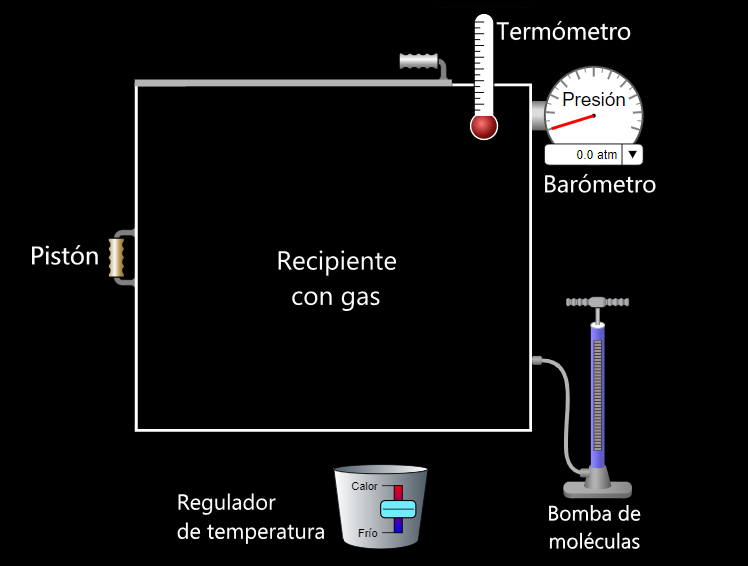
\includegraphics[width= 12cm, height= 7cm]{imag/Materiales.png}
\end{figure}


%=========Procedimiento
\section{Procedimiento}
\begin{enumerate}
    \item Para la primera simulación, trabajamos a una temperatura constante de 300K y un número de partículas pesadas n = 50. Luego variamos el ancho del recipiente (15nm, 13nm, 11nm,
    9nm, 7nm y 5nm). Después registramos cada valor de presión obtenido de la simulación, para cada
    uno de los anchos respectivos.
    Una vez terminada la primera recolección de datos, se repitió la simulación para partículas pesadas y ligeras, ocupando temperaturas constantes de 300K y 600K, y n = 50, n = 100, n = 150
    para cada caso. 

    \item Para la segunda simulación, se trabajó con un número de partículas pesadas n = 50, una
    temperatura inicial de 300K, un recipiente de ancho 10nm  y presión constante entre 5,4atm y 6,3atm.
    Luego se fue variando la temperatura en 150K, 225K, 375K y 450K, con el objetivo de registar las variaciones del ancho del recipiente.
    

    \item   Repetimos la simulación anterior, pero trabajando con un n = 150,  una temperatura inicial de 300K,  un recipiente de ancho 10nm y presión constante entre 17,1atm y 17,9atm. 
    Luego se fue variando la temperatura en 150K, 225K, 375K y 450K, con el objetivo de registar las variaciones del ancho del recipiente. 
    
    \item  Por último, volvemos a realizar la simulación con un n = 250, una temperatura inicial de 300K, un
    recipiente inicial de ancho 10nm y presión constante entre 28,8atm y 29,6atm.
    Luego se fue variando la temperatura en 150K, 225K, 375K y 450K, con el objetivo de registar las variaciones del ancho del recipiente.
   
    
    
\end{enumerate}









%========Resultados








\section{Resultados}
\begin{table}[!h]
 \centering
 \begin{tabular}{|c|c|c|l|} \hline
  n (mol)&  T = 300K        &    T = 600K    &        \\ \hline
   50    & [3.4 - 4.4], 15 & [7.3 - 8.2], 15& P atm, L nm\\ 
         & [4.0 - 5.0], 13 & [8.6 - 9.5], 13& P atm, L nm\\
         & [4.8 - 5.8], 11 & [10.2 - 11.1], 11& P atm, L nm\\ 
         & [6.0 - 7.0],  9 & [12.5 - 13.4],  9& P atm, L nm\\ 
         & [7.9 - 8.8],  7 & [16.2 - 17.1],  7& P atm, L nm\\  
         & [11.2 - 12.1], 5 & [22.9 - 23.8],  5& P atm, L nm\\ \hline
        %%%%%%%%%%%%%%%%%%%%%%%%%%%%%%%%%%%%%%%%%%%%%%%%%%%%%
   100   & [7.3 - 8.2], 15 & [15.1 - 16.0], 15& P atm, L nm\\ 
         & [8.5 - 9.4], 13 & [17.5 - 18.4], 13& P atm, L nm\\
         & [10.2 - 11.1], 11 & [20.9 - 21.7], 11& P atm, L nm\\ 
         & [12.5 - 13.4], 9 & [25.6 - 26.4],  9& P atm, L nm\\ 
         & [16.3 - 17.2], 7 & [32.9 - 33.7],  7& P atm, L nm\\  
         & [22.9 - 23.8] , 5 & [46.3 - 47.1],  5& P atm, L nm\\ \hline
         %%%%%%%%%%%%%%%%%%%%%%%%%%%%%%%%%%%%%%%%%%%%%%%%%%%%%
   150   & [11.2 - 12.1], 15 & [22.9 - 23.8], 15& P atm, L nm\\ 
         & [13.1 - 14.0], 13 & [26.4 - 27.3], 13& P atm, L nm\\
         & [15.5 - 16.3], 11 & [31.4 - 32.2], 11& P atm, L nm\\ 
         & [19.1 - 19.9],  9 & [38.7 - 39.5],  9& P atm, L nm\\ 
         & [24.7 - 25.5],  7 & [49.4 - 50.1],  7& P atm, L nm\\  
         & [34.6 - 35.3],  5 & [69.8 - 70.4],  5& P atm, L nm\\ \hline

   

\end{tabular}
\caption{\label{tab:Pesadas} Datos para partículas pesadas.}
\end{table}

\begin{table}[!h]
 \centering
\begin{tabular}{|c|c|c|l|} \hline
  n (mol)&  T = 300K        &    T = 600K    &        \\ \hline
   50    & [3.7 - 4.9], 15 & [7.6 - 8.1], 15& P atm, L nm\\ 
         & [4.1 - 4.9], 13 & [8.6 - 9.4], 13& P atm, L nm\\
         & [4.9 - 5.8], 11 & [10.2 - 11.0], 11& P atm, L nm\\ 
         & [6.2 - 6.9],  9 & [12.7 - 13.3],  9& P atm, L nm\\ 
         & [7.8 - 8.5],  7 & [16.6 - 17.0],  7& P atm, L nm\\  
         & [11.0 - 12.1], 5 & [23.0 - 23.7],  5& P atm, L nm\\ \hline
        %%%%%%%%%%%%%%%%%%%%%%%%%%%%%%%%%%%%%%%%%%%%%%%%%%%%%
   100   & [7.6 - 8.2], 15 & [15.2 - 15.9], 15& P atm, L nm\\ 
         & [8.5 - 9.4], 13 & [17.6 - 18.3], 13& P atm, L nm\\
         & [10.4 - 11.0], 11 & [20.9 - 21.6], 11& P atm, L nm\\ 
         & [12.6 - 13.1], 9 & [25.5 - 26.3],  9& P atm, L nm\\ 
         & [16.5 - 17.1], 7 & [33.1 - 33.9],  7& P atm, L nm\\  
         & [22.9 - 23.7] , 5 & [46.3 - 47.0],  5& P atm, L nm\\ \hline
         %%%%%%%%%%%%%%%%%%%%%%%%%%%%%%%%%%%%%%%%%%%%%%%%%%%%%
   150   & [11.5 - 12.1], 15 & [23.0 - 23.7], 15& P atm, L nm\\ 
         & [13.1 - 13.6], 13 & [26.5 - 27.3], 13& P atm, L nm\\
         & [15.7 - 16.2], 11 & [31.5 - 32.2], 11& P atm, L nm\\ 
         & [19.1 - 19.7],  9 & [38.5 - 39.1],  9& P atm, L nm\\ 
         & [24.9 - 25.6],  7 & [49.4 - 50.5],  7& P atm, L nm\\  
         & [34.7 - 35.3],  5 & [69.8 - 70.3],  5& P atm, L nm\\ \hline

\end{tabular}
\caption{\label{tab:ligeras} Datos para partículas ligeras.}
\end{table}

 


\begin{table}[!h]
 \centering
 \begin{tabular}{|c|c|l|} \hline
  n (mol)&      P atm      &    T Kelvin, L nm\\ \hline
   50    &                 &             150, 5.0\\
         &  5.8            &             225, 7.5\\
         &                 &             375, 12.5\\
         &                 &             450, 15\\ \hline
            %%%%%%%%%%%%%%%%%%%%%%%%%%%%%%%%%%%%%%%%
   100   &                 &             150, 5.0\\ 
         &  17.5           &             225, 7.5\\
         &                 &             375, 12.5\\ 
         &                 &             450, 15\\ \hline                
            %%%%%%%%%%%%%%%%%%%%%%%%%%%%%%%%%%%%%%%%%
   150   &                 &              150, 5.0\\ 
         &  29.2           &              225, 7.5\\
         &                 &              375, 12.5\\ 
         &                 &              450, 15\\ \hline          

 \end{tabular}
 \caption{\label{tab:V.Ancho} Variación del ancho, con respecto a la temperatura, manteniendo P cte.}    
 \end{table}


\begin{figure}[H]
    \begin{subfigure}
<<<<<<< HEAD
    \raggedright
     \includegraphics[width=8cm, height=6cm]{graficos/grafico1.pdf}
      \caption{\label{fig:ejemplo} mi figura}
=======
    		\raggedright
     	\includegraphics[width=8cm, height=6cm]{graficos/grafico1.pdf}
>>>>>>> e1a4e6a1c4c7f037ddaa4a0eb69ade00fef8a0d9
    \end{subfigure}
    	\begin{subfigure}
    		\raggedright
    		\includegraphics[width=8cm, height=6cm]{graficos/grafico2.pdf}
    	\end{subfigure}
    \begin{subfigure}
    		\raggedright
    		\includegraphics[width=8cm, height=6cm]{graficos/grafico3.pdf}
    	\end{subfigure}
    	\begin{subfigure}
    		\raggedright
    		\includegraphics[width=8cm, height=6cm]{graficos/grafico4.pdf}
    	\end{subfigure}
    	\begin{subfigure}
    		\raggedright
    		\includegraphics[width=8cm, height=6cm]{graficos/grafico5.pdf}
    	\end{subfigure}
    	\begin{subfigure}
    		\raggedright
    		\includegraphics[width=8cm, height=6cm]{graficos/grafico6.pdf}
    	\end{subfigure}
    	\begin{subfigure}
    		\raggedright
    		\includegraphics[width=8cm, height=6cm]{graficos/grafico7.pdf}
    	\end{subfigure}
    	\begin{subfigure}
    		\raggedright
    		\includegraphics[width=8cm, height=6cm]{graficos/grafico8.pdf}
    	\end{subfigure}
    	\begin{subfigure}
    		\raggedright
    		\includegraphics[width=8cm, height=6cm]{graficos/grafico9.pdf}
    	\end{subfigure}
\end{figure}















































%========Analisis
%\section{Análisis}


\newpage
%========Analisis Nosé como poner las respuestas, para que queden separada de la pregunta.
\section{Análisis}
\begin{enumerate}
      \item ¿Qué predice que le sucederá a la presión dentro de un recipiente cuando la temperatura permanece constante pero el volumen cambia?
      \item ¿Qué generalizaciones puede hacer acerca de cómo los cambios de temperatura afectan la presióncuando el volumen en un recipiente permanece constante?
      %\item ¿Qué representa el ́area bajo la curva en un diagrama $(P\-V)$? ¿Cómo se calcula?
\end{enumerate}

%========Conclusión
%\section{Conclusión}












%%%% Bibliografia %%%%%












\end{document}
